\documentclass{standalone}

\usepackage[T1]{fontenc}
\usepackage[utf8]{inputenc}
\usepackage{eulervm}
\usepackage{amsmath}
\usepackage{bm}
\usepackage{tikz}
\usepackage{environ}

\usetikzlibrary{fit}
\usetikzlibrary{patterns}
\usetikzlibrary{arrows}

\usepackage{color}

\definecolor{Comment}{RGB}{97,161,176}

\definecolor{btfGreen}{RGB}{51,160,44}
\definecolor{btfRed}{RGB}{190,60,90}

\definecolor{bleuUni}{RGB}{0, 157, 224}
\definecolor{marronUni}{RGB}{68, 58, 49}
\definecolor{grayMarronUni}{RGB}{60, 60, 60}
\definecolor{grayBleuUni}{RGB}{118, 118, 118}

\definecolor{bluecite}{HTML}{009DE0}

\definecolor{Paired-2}{RGB}{166,206,227}
\definecolor{Paired-1}{RGB}{31,120,180}
\definecolor{Paired-4}{RGB}{178,223,138}
\definecolor{Paired-3}{RGB}{51,160,44}
\definecolor{Paired-6}{RGB}{251,154,153}
\definecolor{Paired-5}{RGB}{227,26,28}
\definecolor{Paired-8}{RGB}{253,191,111}
\definecolor{Paired-7}{RGB}{255,127,0}
\definecolor{Paired-10}{RGB}{202,178,214}
\definecolor{Paired-9}{RGB}{106,61,154}
\definecolor{Paired-12}{RGB}{255,255,153}
\definecolor{Paired-11}{RGB}{177,89,40}
\definecolor{Accent-1}{RGB}{127,201,127}
\definecolor{Accent-2}{RGB}{190,174,212}
\definecolor{Accent-3}{RGB}{253,192,134}
\definecolor{Accent-4}{RGB}{255,255,153}
\definecolor{Accent-5}{RGB}{56,108,176}
\definecolor{Accent-6}{RGB}{240,2,127}
\definecolor{Accent-7}{RGB}{191,91,23}
\definecolor{Accent-8}{RGB}{102,102,102}
\definecolor{Spectral-1}{RGB}{158,1,66}
\definecolor{Spectral-2}{RGB}{213,62,79}
\definecolor{Spectral-3}{RGB}{244,109,67}
\definecolor{Spectral-4}{RGB}{253,174,97}
\definecolor{Spectral-5}{RGB}{254,224,139}
\definecolor{Spectral-6}{RGB}{255,255,191}
\definecolor{Spectral-7}{RGB}{230,245,152}
\definecolor{Spectral-8}{RGB}{171,221,164}
\definecolor{Spectral-9}{RGB}{102,194,165}
\definecolor{Spectral-10}{RGB}{50,136,189}
\definecolor{Spectral-11}{RGB}{94,79,162}
\definecolor{Set1-1}{RGB}{228,26,28}
\definecolor{Set1-2}{RGB}{55,126,184}
\definecolor{Set1-3}{RGB}{77,175,74}
\definecolor{Set1-4}{RGB}{152,78,163}
\definecolor{Set1-5}{RGB}{255,127,0}
\definecolor{Set1-6}{RGB}{255,255,51}
\definecolor{Set1-7}{RGB}{166,86,40}
\definecolor{Set1-8}{RGB}{247,129,191}
\definecolor{Set1-9}{RGB}{153,153,153}
\definecolor{Set2-1}{RGB}{102,194,165}
\definecolor{Set2-2}{RGB}{252,141,98}
\definecolor{Set2-3}{RGB}{141,160,203}
\definecolor{Set2-4}{RGB}{231,138,195}
\definecolor{Set2-5}{RGB}{166,216,84}
\definecolor{Set2-6}{RGB}{255,217,47}
\definecolor{Set2-7}{RGB}{229,196,148}
\definecolor{Set2-8}{RGB}{179,179,179}
\definecolor{Dark2-1}{RGB}{27,158,119}
\definecolor{Dark2-2}{RGB}{217,95,2}
\definecolor{Dark2-3}{RGB}{117,112,179}
\definecolor{Dark2-4}{RGB}{231,41,138}
\definecolor{Dark2-5}{RGB}{102,166,30}
\definecolor{Dark2-6}{RGB}{230,171,2}
\definecolor{Dark2-7}{RGB}{166,118,29}
\definecolor{Dark2-8}{RGB}{102,102,102}
\definecolor{Reds-1}{RGB}{255,245,240}
\definecolor{Reds-2}{RGB}{254,224,210}
\definecolor{Reds-3}{RGB}{252,187,161}
\definecolor{Reds-4}{RGB}{252,146,114}
\definecolor{Reds-5}{RGB}{251,106,74}
\definecolor{Reds-6}{RGB}{239,59,44}
\definecolor{Reds-7}{RGB}{203,24,29}
\definecolor{Reds-8}{RGB}{165,15,21}
\definecolor{Reds-9}{RGB}{103,0,13}
\definecolor{Greens-1}{RGB}{247,252,245}
\definecolor{Greens-2}{RGB}{229,245,224}
\definecolor{Greens-3}{RGB}{199,233,192}
\definecolor{Greens-4}{RGB}{161,217,155}
\definecolor{Greens-5}{RGB}{116,196,118}
\definecolor{Greens-6}{RGB}{65,171,93}
\definecolor{Greens-7}{RGB}{35,139,69}
\definecolor{Greens-8}{RGB}{0,109,44}
\definecolor{Greens-9}{RGB}{0,68,27}
\definecolor{Blues-1}{RGB}{247,251,255}
\definecolor{Blues-2}{RGB}{222,235,247}
\definecolor{Blues-3}{RGB}{198,219,239}
\definecolor{Blues-4}{RGB}{158,202,225}
\definecolor{Blues-5}{RGB}{107,174,214}
\definecolor{Blues-6}{RGB}{66,146,198}
\definecolor{Blues-7}{RGB}{33,113,181}
\definecolor{Blues-8}{RGB}{8,81,156}
\definecolor{Blues-9}{RGB}{8,48,107}


\begin{document}
  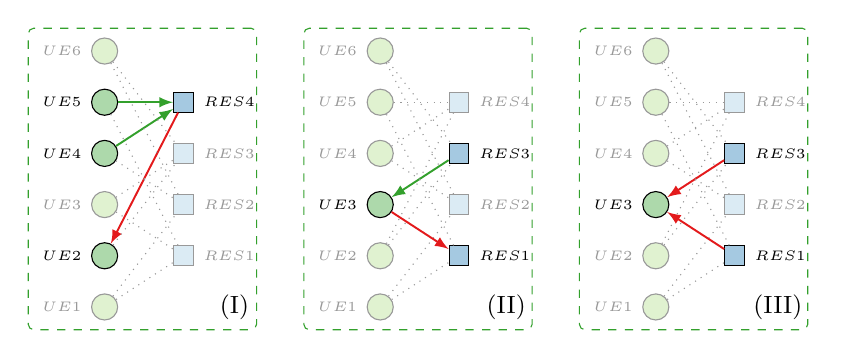
\begin{tikzpicture}[baseline]
    \tikzset{ vn/.style ={draw=black   , circle, minimum width=0.25cm, minimum height=0.25cm, text=black, fill=Paired-3!40 } }
    \tikzset{ cn/.style ={draw=black           , minimum width=0.25cm, minimum height=0.25cm, text=black, fill=Paired-1!40 } }
    \tikzset{ vns/.style={draw=black!40, circle, minimum width=0.25cm, minimum height=0.25cm, text=black, fill=Paired-4!40 } }
    \tikzset{ cns/.style={draw=black!40        , minimum width=0.25cm, minimum height=0.25cm, text=black, fill=Paired-2!40 } }

    \node[vns, label={[black!40]left:\tiny{$UE1$}}] (v1_i) at (0.00, 0.00+0.00) {};
    \node[vn , label={[black   ]left:\tiny{$UE2$}}] (v2_i) at (0.00, 0.25+0.40) {};
    \node[vns, label={[black!40]left:\tiny{$UE3$}}] (v3_i) at (0.00, 0.50+0.80) {};
    \node[vn , label={[black   ]left:\tiny{$UE4$}}] (v4_i) at (0.00, 0.75+1.20) {};
    \node[vn , label={[black   ]left:\tiny{$UE5$}}] (v5_i) at (0.00, 1.00+1.60) {};
    \node[vns, label={[black!40]left:\tiny{$UE6$}}] (v6_i) at (0.00, 1.25+2.00) {};

    \node[cns, label={[black!40]right:\tiny{$RES1$}}] (ca_i) at (1.00, 0.25+0.40) {};
    \node[cns, label={[black!40]right:\tiny{$RES2$}}] (cb_i) at (1.00, 0.50+0.80) {};
    \node[cns, label={[black!40]right:\tiny{$RES3$}}] (cc_i) at (1.00, 0.75+1.20) {};
    \node[cn , label={[black   ]right:\tiny{$RES4$}}] (cd_i) at (1.00, 1.00+1.60) {};

    \draw[dotted, black!40                      ] (v1_i) -- (ca_i);
    \draw[dotted, black!40                      ] (v1_i) -- (cb_i);
    \draw[dotted, black!40                      ] (v2_i) -- (cc_i);
    \draw[<-,>=latex, Paired-5, line width=0.7pt] (v2_i) -- (cd_i);
    \draw[dotted, black!40                      ] (v3_i) -- (ca_i);
    \draw[dotted, black!40                      ] (v3_i) -- (cc_i);
    \draw[dotted, black!40                      ] (v4_i) -- (cb_i);
    \draw[->,>=latex, Paired-3, line width=0.7pt] (v4_i) -- (cd_i);
    \draw[dotted, black!40                      ] (v5_i) -- (ca_i);
    \draw[->,>=latex, Paired-3, line width=0.7pt] (v5_i) -- (cd_i);
    \draw[dotted, black!40                      ] (v6_i) -- (cb_i);
    \draw[dotted, black!40                      ] (v6_i) -- (cc_i);

    \node (i) at (1.65, 0.00+0.00) {\small{(I)}};

    \node[draw=Paired-3, rounded corners=2pt, minimum width=2.9cm, dashed, fit=(v1_i) (v6_i) (ca_i) (cd_i)] {};

    \newcommand\xshft{3.5}

    \node[vns, label={[black!40]left:\tiny{$UE1$}}] (v1_ii) at (\xshft+0.00, 0.00+0.00) {};
    \node[vns, label={[black!40]left:\tiny{$UE2$}}] (v2_ii) at (\xshft+0.00, 0.25+0.40) {};
    \node[vn , label={[black   ]left:\tiny{$UE3$}}] (v3_ii) at (\xshft+0.00, 0.50+0.80) {};
    \node[vns, label={[black!40]left:\tiny{$UE4$}}] (v4_ii) at (\xshft+0.00, 0.75+1.20) {};
    \node[vns, label={[black!40]left:\tiny{$UE5$}}] (v5_ii) at (\xshft+0.00, 1.00+1.60) {};
    \node[vns, label={[black!40]left:\tiny{$UE6$}}] (v6_ii) at (\xshft+0.00, 1.25+2.00) {};

    \node[cn , label={[black   ]right:\tiny{$RES1$}}] (ca_ii) at (\xshft+1.00, 0.25+0.40) {};
    \node[cns, label={[black!40]right:\tiny{$RES2$}}] (cb_ii) at (\xshft+1.00, 0.50+0.80) {};
    \node[cn , label={[black   ]right:\tiny{$RES3$}}] (cc_ii) at (\xshft+1.00, 0.75+1.20) {};
    \node[cns, label={[black!40]right:\tiny{$RES4$}}] (cd_ii) at (\xshft+1.00, 1.00+1.60) {};

    \draw[dotted, black!40                      ] (v1_ii) -- (ca_ii);
    \draw[dotted, black!40                      ] (v1_ii) -- (cb_ii);
    \draw[dotted, black!40                      ] (v2_ii) -- (cc_ii);
    \draw[dotted, black!40                      ] (v2_ii) -- (cd_ii);
    \draw[->,>=latex, Paired-5, line width=0.7pt] (v3_ii) -- (ca_ii);
    \draw[<-,>=latex, Paired-3, line width=0.7pt] (v3_ii) -- (cc_ii);
    \draw[dotted, black!40                      ] (v4_ii) -- (cb_ii);
    \draw[dotted, black!40                      ] (v4_ii) -- (cd_ii);
    \draw[dotted, black!40                      ] (v5_ii) -- (ca_ii);
    \draw[dotted, black!40                      ] (v5_ii) -- (cd_ii);
    \draw[dotted, black!40                      ] (v6_ii) -- (cb_ii);
    \draw[dotted, black!40                      ] (v6_ii) -- (cc_ii);

    \node (ii) at (\xshft+1.60, 0.00+0.00) {\small{(II)}};

    \node[draw=Paired-3, rounded corners=2pt, minimum width=2.9cm, dashed, fit=(v1_ii) (v6_ii) (ca_ii) (cd_ii)] {};

    \node[vns, label={[black!40]left:\tiny{$UE1$}}] (v1_iii) at (\xshft+\xshft+0.00, 0.00+0.00) {};
    \node[vns, label={[black!40]left:\tiny{$UE2$}}] (v2_iii) at (\xshft+\xshft+0.00, 0.25+0.40) {};
    \node[vn , label={[black   ]left:\tiny{$UE3$}}] (v3_iii) at (\xshft+\xshft+0.00, 0.50+0.80) {};
    \node[vns, label={[black!40]left:\tiny{$UE4$}}] (v4_iii) at (\xshft+\xshft+0.00, 0.75+1.20) {};
    \node[vns, label={[black!40]left:\tiny{$UE5$}}] (v5_iii) at (\xshft+\xshft+0.00, 1.00+1.60) {};
    \node[vns, label={[black!40]left:\tiny{$UE6$}}] (v6_iii) at (\xshft+\xshft+0.00, 1.25+2.00) {};

    \node[cn , label={[black   ]right:\tiny{$RES1$}}] (ca_iii) at (\xshft+\xshft+1.00, 0.25+0.40) {};
    \node[cns, label={[black!40]right:\tiny{$RES2$}}] (cb_iii) at (\xshft+\xshft+1.00, 0.50+0.80) {};
    \node[cn , label={[black   ]right:\tiny{$RES3$}}] (cc_iii) at (\xshft+\xshft+1.00, 0.75+1.20) {};
    \node[cns, label={[black!40]right:\tiny{$RES4$}}] (cd_iii) at (\xshft+\xshft+1.00, 1.00+1.60) {};

    \draw[dotted, black!40                      ] (v1_iii) -- (ca_iii);
    \draw[dotted, black!40                      ] (v1_iii) -- (cb_iii);
    \draw[dotted, black!40                      ] (v2_iii) -- (cc_iii);
    \draw[dotted, black!40                      ] (v2_iii) -- (cd_iii);
    \draw[<-,>=latex, Paired-5, line width=0.7pt] (v3_iii) -- (ca_iii);
    \draw[<-,>=latex, Paired-5, line width=0.7pt] (v3_iii) -- (cc_iii);
    \draw[dotted, black!40                      ] (v4_iii) -- (cb_iii);
    \draw[dotted, black!40                      ] (v4_iii) -- (cd_iii);
    \draw[dotted, black!40                      ] (v5_iii) -- (ca_iii);
    \draw[dotted, black!40                      ] (v5_iii) -- (cd_iii);
    \draw[dotted, black!40                      ] (v6_iii) -- (cb_iii);
    \draw[dotted, black!40                      ] (v6_iii) -- (cc_iii);

    \node (iii) at (\xshft+\xshft+1.55, 0.00+0.00) {\small{(III)}};

    \node[draw=Paired-3, rounded corners=2pt, minimum width=2.9cm, dashed, fit=(v1_iii) (v6_iii) (ca_iii) (cd_iii)] {};
  \end{tikzpicture}
\end{document}